\documentclass{article}

% ICML 2026 style. Place icml2026.sty, icml2026.bst and fancyhdr.sty in this directory
% (from the official icml2026.zip) before compiling on Overleaf.
\usepackage{microtype}
\usepackage{graphicx}
\usepackage{booktabs}
\usepackage{amsmath}
\usepackage{amssymb}
\usepackage{multirow}
\usepackage{url}
\usepackage[hidelinks]{hyperref}
\usepackage{xurl}                      % URLs may break at any character
\urlstyle{same}                        % URLs in body font, not wide monospace
\DeclareUrlCommand\file{\urlstyle{tt}} % breakable monospace file names
\setlength{\emergencystretch}{1.5em}   % avoid lines overrunning the narrow columns
\newcommand{\theHalgorithm}{\arabic{algorithm}}

\usepackage[accepted]{icml2026}
% Remove the default "Proceedings of ICML 2026" notice: this is a course report.
\makeatletter\renewcommand{\Notice@String}{}
% First-page footnote: affiliation only, no "Correspondence to" line.
\renewcommand{\printAffiliationsAndNotice}[1]{\global\icml@noticeprintedtrue
  {\let\thefootnote\relax\footnotetext{\hspace*{-\footnotesep}#1}}}
\makeatother

%% ===================================================================
%% EDIT THIS ONE LINE with your GitHub repository URL before submitting.
\newcommand{\repourl}{https://github.com/pruthav23/CHE629_Optimus5Prime.git}
%% ===================================================================

\icmltitlerunning{Beyond Optimus 5-Prime: A CNN--Attention Hybrid for 5'UTR Translation Control}

\begin{document}

\twocolumn[
\icmltitle{Beyond Optimus 5-Prime: Reproduction and a\\
CNN--Attention Hybrid for 5$'$UTR Translation Control}

\begin{icmlauthorlist}
\icmlauthor{Tushar Srikrishna Sridhar (231103)}{}
\icmlauthor{Anika Gupta (230137)}{}
\icmlauthor{Prutha Vinay (230807)}{}
\end{icmlauthorlist}
% Single affiliation: no superscript markers. The affiliation is printed
% in the first-page footnote via \printAffiliationsAndNotice below.

\icmlkeywords{5'UTR, translation, mean ribosome load, convolutional networks, attention, reproducibility}

\vskip 0.3in
]

\printAffiliationsAndNotice{Indian Institute of Technology Kanpur, Kanpur, India.}

\begin{abstract}
The 5$'$ untranslated region (5$'$UTR) of a messenger RNA controls how efficiently that
message is translated, which makes it a central design variable for mRNA therapeutics.
\citet{sample2019} introduced \emph{Optimus 5-Prime}, a convolutional network that predicts
mean ribosome load (MRL) from a 50\,nt 5$'$UTR and explains 93\% of the variance of a
massively parallel reporter assay. We reproduce that result from scratch in PyTorch~\citep{paszke2019}
($r^2=0.919\pm0.006$ over three seeds), first validating the whole pipeline on a
\emph{synthetic} dataset whose generative rules we control, and we benchmark the model
against three alternatives under one shared protocol. We then address one limitation of the
original work: it evaluates a single architecture at a single data size, so it is not known
whether the convolutional inductive bias is the right one for this task or merely a
sufficient one. We run a controlled architecture $\times$ data-regime study at matched
parameter counts and matched tuning budgets, and find that a CNN+attention hybrid reaches
$r^2=0.942\pm0.001$ --- clearly above the published CNN and the strongest model in our
comparison --- while a pure transformer on the same input fails outright in low-data regimes.
In-silico mutagenesis shows that the hybrid refines the grammar the CNN already learns rather
than learning a different one. Code, trained weights and all per-run metrics:
\url{\repourl}.
\end{abstract}

\section{Introduction}
\label{sec:intro}

Translation of a eukaryotic mRNA begins when the small ribosomal subunit binds near the
5$'$ cap and scans along the transcript until it recognises a start codon. Everything the
scanning ribosome encounters before the main coding sequence (CDS) therefore shapes how much
protein the message yields: upstream AUG codons (uAUGs) that capture scanning ribosomes,
upstream open reading frames (uORFs) that terminate before the CDS, the Kozak sequence
context around each start codon, and secondary structure that impedes scanning~\citep{kozak1986}. The 5$'$UTR
is thus a compact, highly interpretable regulatory element, and one that can be engineered:
tuning a 50\,nt sequence is a practical lever for mRNA vaccine and therapeutic design.

\citet{sample2019} made this problem tractable for machine learning. They built a massively
parallel reporter assay (MPRA) over a library of 280{,}000 random 50\,nt 5$'$UTRs, measured
the \emph{mean ribosome load} (MRL) of each by polysome profiling, and trained a
three-layer convolutional network, \emph{Optimus 5-Prime}, to predict MRL from one-hot
encoded sequence. The model explains 93\% of held-out variance and generalises to human
5$'$UTRs and to clinical variants.

\paragraph{Contributions.}
\begin{enumerate}\itemsep2pt
\item A faithful PyTorch reproduction ($r^2=0.919\pm0.006$ vs.\ 0.93 published), verified by
loading the authors' own Keras weights into our implementation ($r^2=0.934$).
\item A synthetic 5$'$UTR simulator with known rules and a computable noise ceiling, used to
validate the pipeline and to test \emph{which} rules each model actually learns.
\item A three-benchmark comparison under one protocol, reporting regression and
classification metrics (accuracy, macro precision/recall/F1, confusion matrices).
\item One focused extension: a controlled architecture $\times$ data-regime study, at
matched parameter counts and matched tuning budgets, yielding a CNN+attention hybrid that
improves on the published architecture ($r^2=0.942\pm0.001$ against $0.922\pm0.002$ for the
CNN under the identical protocol), together with an in-silico mutagenesis check that the
hybrid refines rather than replaces the grammar the CNN learns.
\end{enumerate}

\section{The Original Work}
\label{sec:paper}

\paragraph{Biological problem.} Given a 50\,nt 5$'$UTR immediately upstream of a fixed
reporter CDS, predict how heavily ribosomes load onto that transcript. MRL is a scalar
summary of the polysome distribution: transcripts are fractionated by the number of bound
ribosomes, and
$\mathrm{MRL} = \sum_{k} k \, p_k$,
where $p_k$ is the fraction of that UTR's reads in polysome fraction $k$. High MRL means
efficient translation initiation.

\paragraph{Dataset.} A library of random 50-mers was cloned upstream of eGFP, transcribed
\emph{in vitro}, transfected into HEK293T cells, and separated over a sucrose gradient into
14 fractions, each sequenced. After filtering, the 280{,}000 most deeply sequenced UTRs were
retained. The authors also produced the same library with uridine replaced by pseudouridine
($\Psi$) or N1-methylpseudouridine (m1$\Psi$) --- the modified nucleotides used in mRNA
vaccines~\citep{kariko2008} --- an mCherry-CDS library, a designed library containing 35{,}212 human 5$'$UTRs
and 3{,}577 ClinVar variants, and a variable-length (25--100\,nt) library.

\paragraph{Deep learning formulation.} Each UTR is one-hot encoded to a $50\times4$ matrix.
Optimus 5-Prime applies three 1-D convolutions (120 filters, width 8, \texttt{same} padding,
ReLU), flattens, and passes through a 40-unit dense layer with 20\% dropout to a single
linear output. It is trained with MSE on standardised MRL using Adam ($10^{-3}$), batch 128,
for three epochs --- the authors stop there because the model begins to overfit. Performance
is reported as $r^2$, the \emph{squared Pearson correlation} between observed and predicted
MRL on the 20{,}000 most deeply sequenced UTRs, which are held out.

\section{Data and Experimental Setup}
\label{sec:data}

\subsection{Real data and splits}
We use GEO accession GSE114002. Following the original protocol exactly, UTRs are sorted by
total read count, the top 280{,}000 are kept, the \textbf{top 20{,}000 form the test set},
and the remaining \textbf{260{,}000 form the training pool}. Because deeper sequencing means
less measurement noise, this makes the test set the cleanest part of the data; we therefore
also report a random-split control (Section~\ref{sec:arch}).

The published recipe has no validation set: it fixes three epochs. For every experiment
beyond the literal reproduction we carve a validation split from the training pool
(10\% at full data, 20\% in small-data regimes) and use it for \emph{all} model selection ---
learning rate, dropout, and early stopping. The 20{,}000 test UTRs are never used for any
choice, and training subsets are drawn only from the training pool. Subset indices and seeds
are saved to disk.

\paragraph{Noise ceiling.} Because two biological replicates exist per chemistry, the best
$r^2$ any model can achieve against replicate 1 equals the Pearson correlation between
replicates: 0.971 (U), 0.916 ($\Psi$), 0.865 (m1$\Psi$). Every experiment in this report
uses the unmodified (U) library, so 0.971 bounds every number we report on real data.

\subsection{Synthetic dataset}
\label{sec:synth}
The paper's library is often called ``synthetic'', but only the \emph{sequences} are
designed; the MRL labels are real measurements with real noise. To validate our pipeline
before using real data, we built a genuinely synthetic dataset of 280{,}000 random 50-mers
with labels generated from rules we control, following a leaky-scanning model:
\begin{equation}
\mathrm{MRL}_{\text{true}} = 1 + 7 \cdot e^{0.025\,\mathrm{MFE}} \prod_{i \in \mathcal{A}} (1 - r_i),
\end{equation}
where $\mathcal{A}$ is the set of upstream AUGs and $r_i = b_i \cdot \kappa_i$. The base
repression $b_i$ depends on what the uAUG does: 0.40 if an in-frame stop precedes the CDS
(a self-contained uORF, permitting reinitiation), 0.75 if it is out of frame with no stop
(an overlapping ORF), and 0.12 if it reads in frame into the CDS (an N-terminal extension).
The Kozak factor $\kappa_i = 0.35 + 0.35\,[\,-3 \in \{A,G\}\,] + 0.30\,[\,+4 = G\,]$.
Minimum free energy (MFE) is computed with ViennaRNA~\citep{lorenz2011}. Observed labels add
$\mathcal{N}(0, 0.45^2)$, which fixes a computable noise ceiling of $r^2 = 0.918$.

This dataset serves three purposes: it validates preprocessing and training code against a
known answer; it bounds achievable performance; and, because we know the planted rules, it
lets us ask \emph{which} rules a model has learned rather than only how well it scores.

\section{Reproduction}
\label{sec:repro}

\begin{figure}[t]
\centering
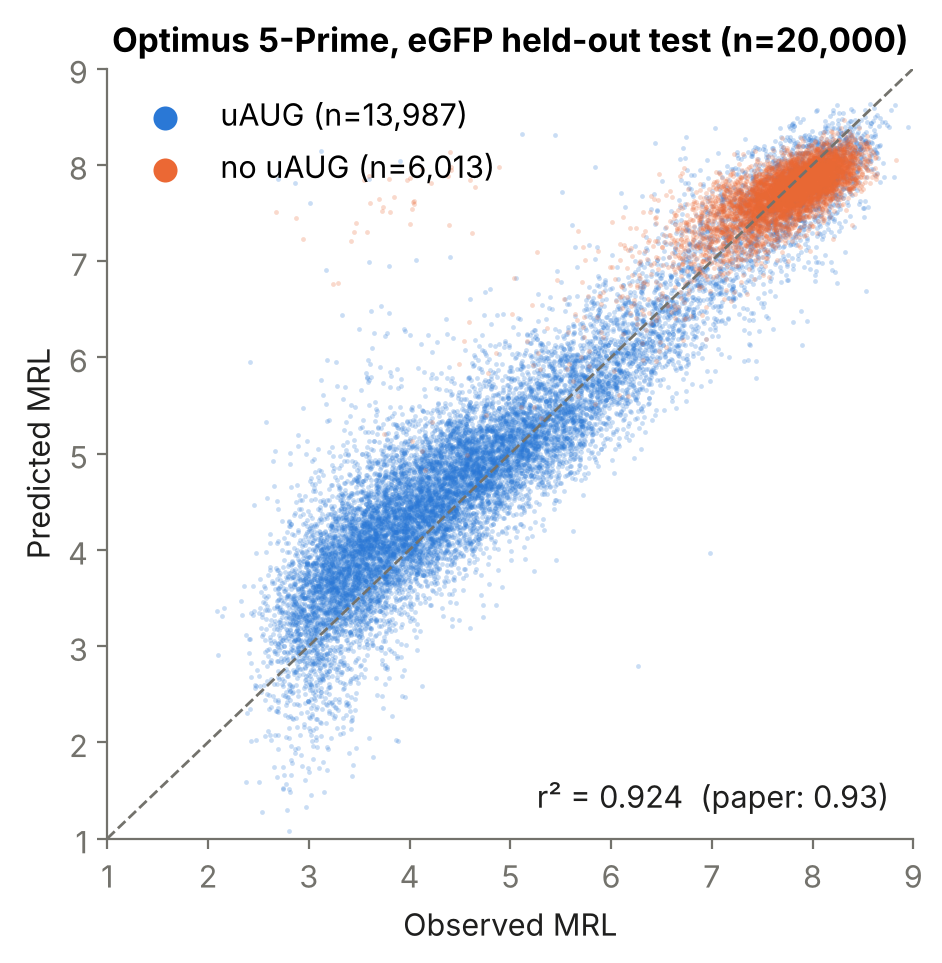
\includegraphics[width=\columnwidth]{figs/fig2b_test_scatter.png}
\caption{Reproduction of the paper's Figure~2b. Predicted vs.\ observed MRL on the 20{,}000
held-out UTRs, coloured by presence of an upstream AUG. Our from-scratch model reaches
$r^2=0.924$ on this seed (published: 0.93). The uAUG-free sequences (orange) occupy the
high-MRL mode, as expected biologically.}
\label{fig:repro}
\end{figure}

\paragraph{Pipeline validation.} Before training anything, we loaded the authors' released
Keras weights (\file{main_MRL_model.hdf5}) into our PyTorch module and evaluated on our
preprocessed test set, obtaining $r^2 = 0.934$. This confirms that our data processing,
one-hot encoding, and architecture match theirs exactly. One subtlety: Keras \texttt{same}
padding for an even kernel ($k=8$) pads 3 on the left and 4 on the right, which must be
replicated for the weights to transfer.

\paragraph{Synthetic first, then real.} On the synthetic dataset the CNN reaches
$r^2 = 0.856 \pm 0.006$ against a noise ceiling of 0.918. Crucially, in-silico insertion of
a single ATG into uAUG-free sequences shows the model recovers the planted rules
quantitatively (Figure~\ref{fig:ism}): mean predicted $\Delta$MRL of $-0.43$ / $-1.38$ /
$-2.39$ for in-frame / uORF / overlapping-ORF insertions, against ground truth $-0.40$ /
$-1.36$ / $-2.52$ ($r = 0.95$ across all insertions). The model has learned the frame logic,
not merely ``ATG is bad''.

On the real data, training from scratch with the published recipe gives
$r^2 = 0.919 \pm 0.006$ over three seeds (0.924, 0.921, 0.910), against the published 0.93
(Figure~\ref{fig:repro}). The residual gap is consistent with seed variance: with only three
epochs, no learning-rate schedule and no early stopping, run-to-run spread is $\approx 0.01$,
and the paper reports a single run. Under our proper train/validation/test protocol with
early stopping the same architecture gives $r^2 = 0.922 \pm 0.002$.

\paragraph{Biological sanity checks.} Independently of the model, the data reproduce the
published frame effect: among single-uAUG UTRs, out-of-frame uAUGs depress MRL to
$\approx 4.5$--$5.5$ while in-frame uAUGs are far milder and approach uAUG-free levels close
to the CDS. We also reproduce the human-UTR evaluation (Figure~4a of the paper) at
$r^2 = 0.784$; the published 0.81 uses a \emph{retrained} model whose weights and exact
recipe are not in the authors' repository. The authors' own original model scores 0.789 on
our pipeline, so the gap is attributable to that missing model rather than to our
implementation.

\begin{figure}[t]
\centering
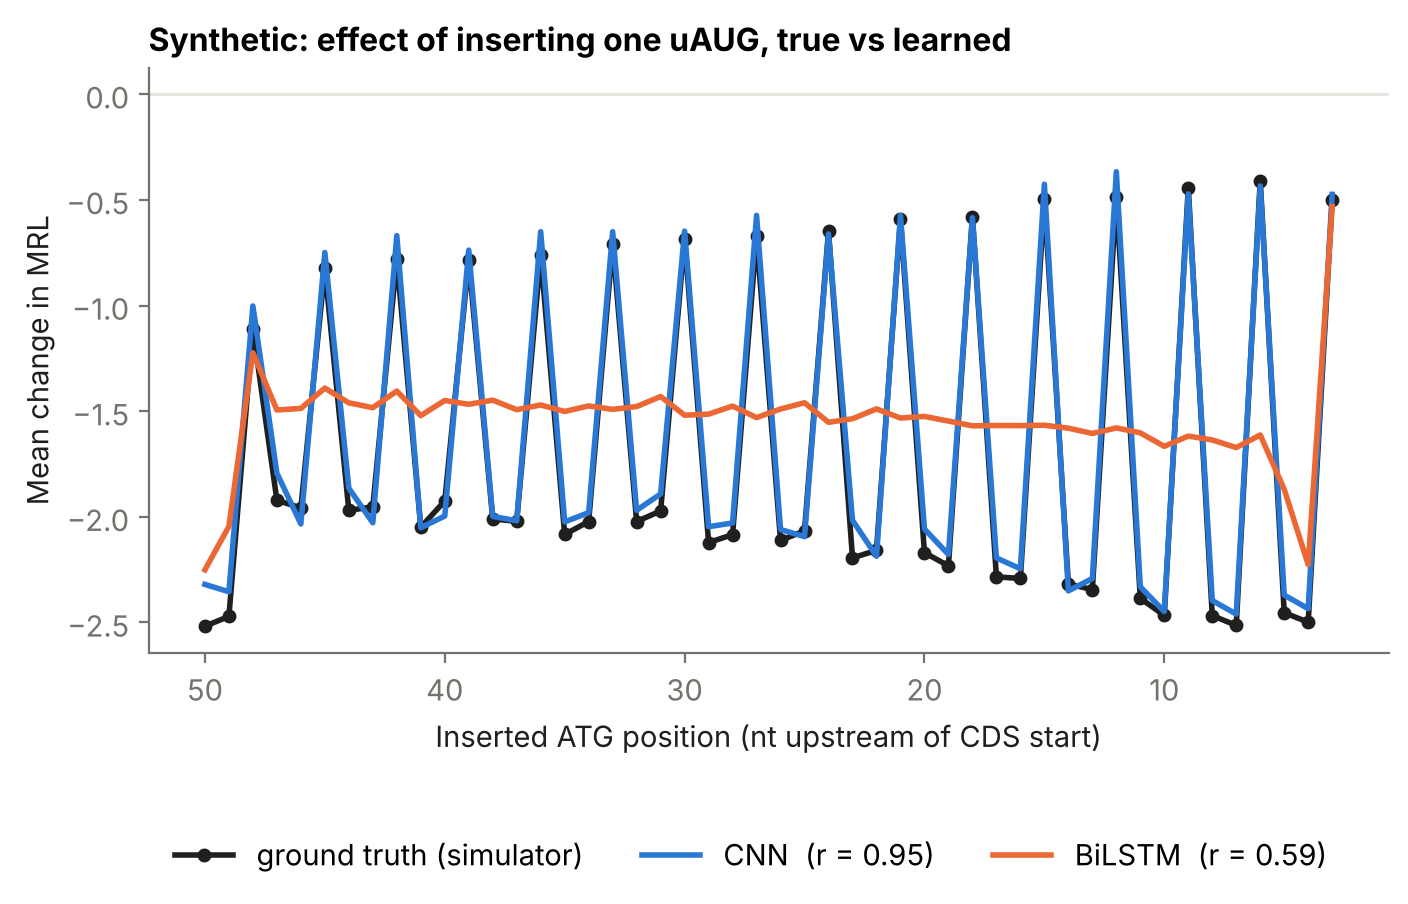
\includegraphics[width=\columnwidth]{figs/synth_atg_insertion.png}
\caption{Rule recovery on synthetic data. A single ATG is inserted at every position of 400
uAUG-free test UTRs and the predicted change in MRL is compared with the simulator's true
change. The CNN tracks the ground truth, including the three-nucleotide frame periodicity;
the BiLSTM learns only that ATG is repressive.}
\label{fig:ism}
\end{figure}

\section{Benchmark Comparison}
\label{sec:bench}

\begin{figure}[t]
\centering
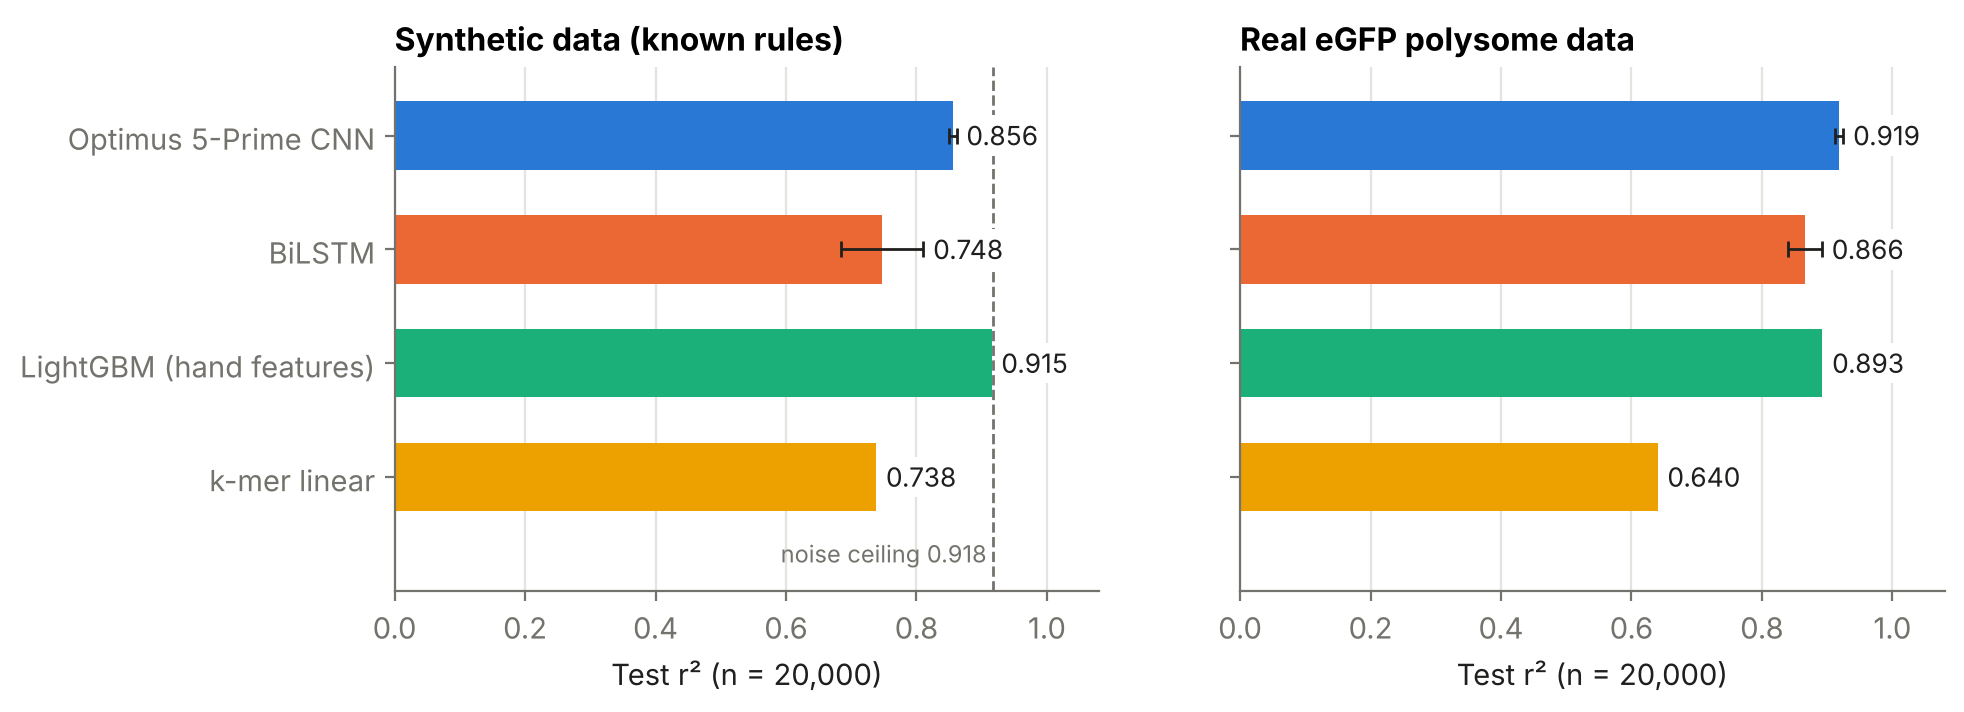
\includegraphics[width=\columnwidth]{figs/r2_synth_vs_real.png}
\caption{Benchmark comparison on synthetic data (left, with computable noise ceiling) and
real eGFP data (right). LightGBM's synthetic score is near-oracle because its hand-crafted
features encode the very rules the simulator plants.}
\label{fig:bench}
\end{figure}

We compare Optimus 5-Prime against three benchmarks, all trained and evaluated under the
identical protocol of Section~\ref{sec:data}:
\begin{itemize}\itemsep2pt
\item \textbf{Position-specific $k$-mer linear model} ($k=1\ldots6$, ridge regression) ---
the paper's own baseline;
\item \textbf{LightGBM}~\citep{ke2017} on hand-crafted features: uAUG counts by functional type, best Kozak
context per type, stop-codon counts per frame, distance of first/last uAUG, GC content, MFE,
and 1--3-mer counts (98 features);
\item \textbf{BiLSTM}~\citep{hochreiter1997} (bidirectional LSTM, mean+max pooling) --- a different deep-learning
family on the same one-hot input.
\end{itemize}

Because the task is regression but the rubric calls for classification metrics, we
additionally bin MRL into \textbf{tertiles of the training distribution} (low $<5.98 \le$
medium $<7.63 \le$ high) and report accuracy and macro-averaged precision, recall and F1,
with confusion matrices. Table~\ref{tab:bench} gives the unified comparison on real data and
Figure~\ref{fig:cm} the confusion matrices; Figure~\ref{fig:bench} contrasts synthetic and
real performance.

\begin{table*}[t]
\caption{Unified comparison on the real eGFP held-out test set ($n=20{,}000$).
Rows above the rule are the reproduction and the three benchmarks; rows below are the
architectures compared in Section~\ref{sec:arch}. Classification metrics use training-set
tertiles of MRL; precision, recall and F1 are macro-averaged. Mean $\pm$ sd over seeds where
more than one seed was run.}
\label{tab:bench}
\vskip 0.1in
\begin{center}
\begin{small}
\setlength{\tabcolsep}{3.4pt}
\begin{tabular}{llcccccccc}
\toprule
Model & Role & Seeds & $r^2$ & Spearman & RMSE & Accuracy & Precision & Recall & F1 \\
\midrule
Optimus 5-Prime CNN & reproduction & 3 & $0.919${\scriptsize$\pm.006$} & 0.942 & 0.547 & 0.869 & 0.822 & 0.822 & 0.819 \\
$k$-mer linear & benchmark & 1 & 0.640 & 0.832 & 1.155 & 0.696 & 0.723 & 0.659 & 0.636 \\
LightGBM (hand features) & benchmark & 1 & 0.893 & 0.922 & 0.620 & 0.848 & 0.795 & 0.791 & 0.791 \\
BiLSTM & benchmark & 3 & $0.866${\scriptsize$\pm.026$} & 0.907 & 0.746 & 0.819 & 0.773 & 0.769 & 0.763 \\
\midrule
Transformer & ours & 3 & $0.728${\scriptsize$\pm.012$} & 0.835 & 1.013 & 0.713 & 0.704 & 0.655 & 0.635 \\
\textbf{CNN + attention hybrid} & ours & 3 & $\mathbf{0.942}${\scriptsize$\pm.001$} & \textbf{0.955} & \textbf{0.454} & \textbf{0.886} & \textbf{0.839} & \textbf{0.843} & \textbf{0.841} \\
\bottomrule
\end{tabular}
\end{small}
\end{center}
\vskip -0.1in
\end{table*}

\begin{figure*}[t]
\centering
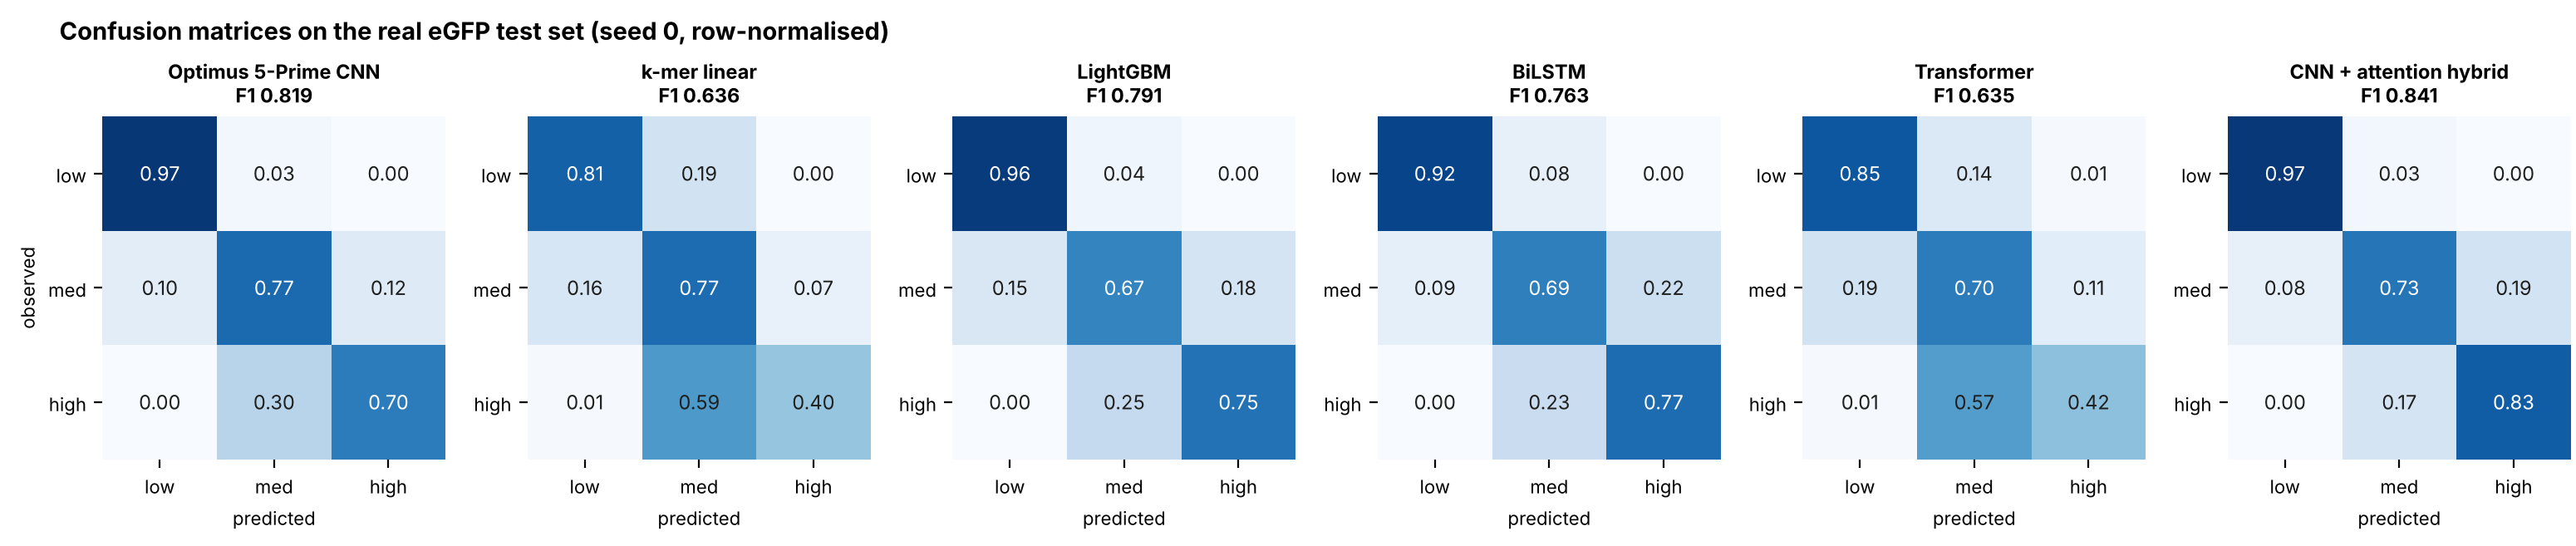
\includegraphics[width=\textwidth]{figs/confusion_matrices_6models.png}
\caption{Row-normalised confusion matrices on the real test set (seed 0) for MRL binned into
training-set tertiles. Every model finds the low-MRL class easiest, because a single uAUG is
a strong and easily learned signal; the high class is hardest, requiring the absence of
repressive elements \emph{and} favourable structure. The CNN+attention hybrid (rightmost) is
the only model whose recall on the high-MRL class exceeds 0.80.}
\label{fig:cm}
\end{figure*}

\paragraph{Interpretation.} Three observations matter more than the ranking itself.

\emph{(i) The deep model earns its place, but not by as much as the paper's baseline
suggests.} The published comparison is against a $k$-mer linear model (0.66 published, 0.640
reproduced here). A properly tuned gradient-boosted model on biologically informed features
reaches 0.893 --- far closer to the CNN. The honest claim is that the CNN beats strong
feature engineering by $\approx 0.03$ $r^2$ while requiring no domain features at all.

\emph{(ii) LightGBM's synthetic score is near-oracle and should not be read as a win.} On
synthetic data it scores 0.915 against the ceiling of 0.918, but its features (uAUG type,
Kozak strength, MFE) are precisely the quantities the simulator uses. This is exactly the
diagnostic value of the synthetic set: it separates ``learned the task'' from ``was handed
the answer''.

\emph{(iii) Error structure is biologically sensible.} All confusion matrices are strongly
diagonal with errors confined to adjacent classes; no model confuses low with high MRL. The
low class is recovered best (0.92--0.97 recall for the stronger models), consistent with a
single out-of-frame uAUG being a near-deterministic repressive signal.

\section{The CNN--Attention Hybrid}
\label{sec:novelty}

The reproduction shows that the published CNN is a strong model, and the benchmark
comparison narrows its margin over well-tuned feature engineering to $\approx0.03$ $r^2$
(Section~\ref{sec:bench}). Neither result tells us whether the convolutional inductive bias
is the \emph{right} one for this task or merely a sufficient one, because the original work
evaluates a single architecture at a single data size. There is a concrete reason to ask. A
convolutional stack reads a fixed receptive field and can only compose distant positions
through depth, whereas the biology is explicitly about interaction between distant positions:
how much a given uAUG represses depends on its Kozak context, on whether a stop codon occurs
later in frame, and on structure elsewhere in the 50\,nt window. Self-attention models such
interactions directly, which raises two questions --- whether attention helps at all here, and
whether it helps on its own or only on top of a convolutional stem.

We therefore run one controlled architecture $\times$ data-regime study, and it yields the
single extension we propose: a hybrid that feeds a convolutional stem into a transformer
encoder. Everything else about the setup --- the data, the splits, the test set and the
evaluation protocol --- is unchanged from Section~\ref{sec:data}, so the comparison against
the reproduced CNN is like-for-like.

\subsection{Architectures across data regimes}
\label{sec:arch}

\begin{figure}[t]
\centering
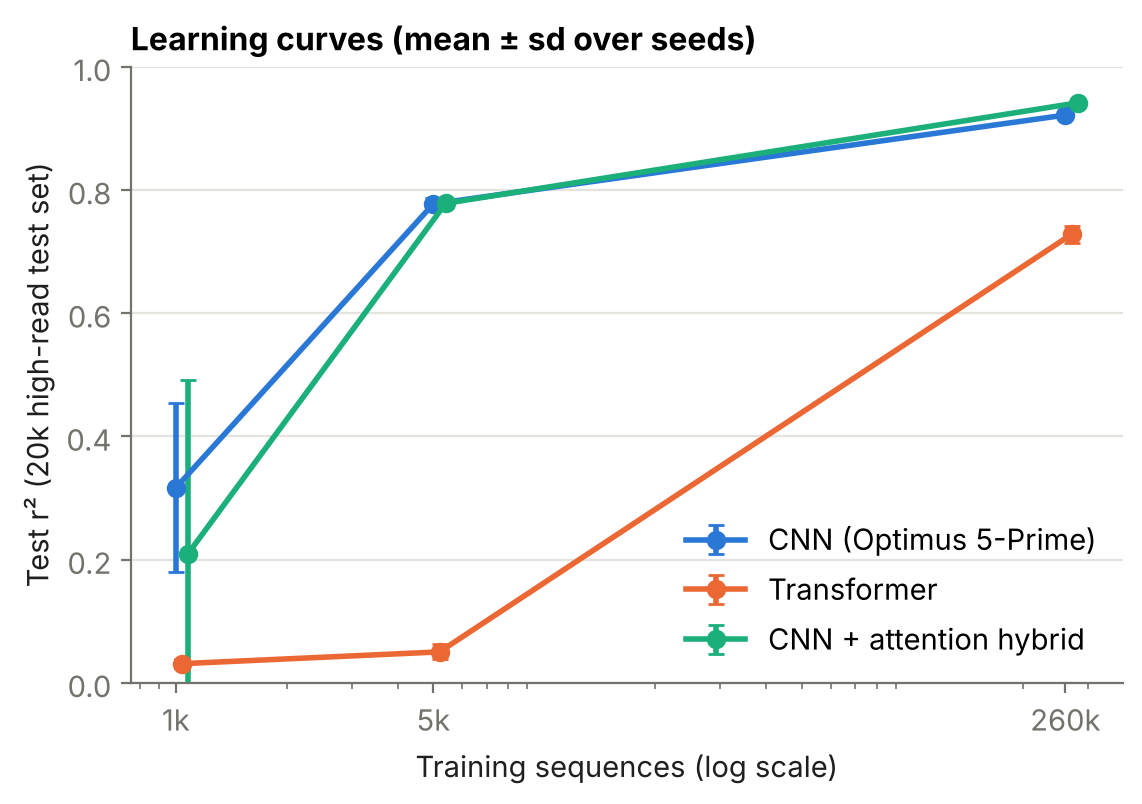
\includegraphics[width=\columnwidth]{figs/B_learning_curves.png}
\caption{Learning curves. Parameter counts are matched (475k / 457k / 421k) and every
architecture receives the same tuning budget, early-stopping rule and seeds at each data
size. The transformer's full-data point is budget-limited (see text).}
\label{fig:lc}
\end{figure}

The paper evaluates one architecture at one data size. We compare three at
$\{1\mathrm{k}, 5\mathrm{k}, 260\mathrm{k}\}$ training sequences: the CNN (475k parameters),
a pre-LN transformer encoder~\citep{vaswani2017} over the 50 positions with learned
positional embeddings and mean pooling (457k), and a hybrid of two convolutional layers feeding a three-layer
transformer (421k). Fairness controls: matched parameter counts, an identical tuning grid
per architecture per data size (learning rate $\times$ dropout, selected on validation),
the same early-stopping rule, five seeds at 1k/5k and three at full data, and nested random
subsets drawn only from the training pool.

\begin{table}[t]
\caption{Test $r^2$ by architecture and training-set size (mean $\pm$ sd; five seeds at
1k/5k, three at 260k). $^\dagger$All three full-data transformer runs hit the 15-epoch cap
while validation loss was still falling, so this value is budget-limited rather than a
converged ceiling.}
\label{tab:arch}
\vskip 0.1in
\begin{center}
\begin{small}
\begin{tabular}{lccc}
\toprule
Train size & CNN & Transformer & Hybrid \\
\midrule
1{,}000   & $\mathbf{0.317}${\scriptsize$\pm.123$} & $0.031${\scriptsize$\pm.007$} & $0.210${\scriptsize$\pm.251$} \\
5{,}000   & $\mathbf{0.778}${\scriptsize$\pm.009$} & $0.050${\scriptsize$\pm.011$} & $\mathbf{0.778}${\scriptsize$\pm.005$} \\
260{,}000 & $0.922${\scriptsize$\pm.002$} & $0.728^\dagger${\scriptsize$\pm.012$} & $\mathbf{0.942}${\scriptsize$\pm.001$} \\
\bottomrule
\end{tabular}
\end{small}
\end{center}
\vskip -0.1in
\end{table}

Table~\ref{tab:arch} and Figure~\ref{fig:lc} give the result. \textbf{The hybrid is the best
model at full data}, reaching $r^2 = 0.942 \pm 0.001$ --- above the published CNN on all
three seeds, with fewer parameters and lower RMSE (0.454 vs.\ 0.522). The convolutional stem
supplies the local motif prior that attention otherwise has to discover, while self-attention
adds the long-range composition the CNN lacks.

\textbf{The pure transformer fails, and the failure is informative.} At 1k and 5k it cannot
fit even its training set. We verified this is not an implementation bug using training data
only: changing the learning rate does not help, replacing the learned positional embedding
with a sinusoidal one does not help, and the identical encoder behind a convolutional stem
(the hybrid) trains normally. At full data it sits on a plateau for roughly eight epochs
($\approx14$k updates) before breaking out, and all three runs were stopped by the shared
15-epoch cap while still improving. Learning a motif such as ATG from single-nucleotide
tokens through attention alone requires far more optimisation steps than the convolutional
prior needs.

\paragraph{Sensitivity and controls.} Because the hybrid is bimodal at 1k (either
$\approx0.65$ or $\approx0.04$, depending on whether it escapes the initial plateau), we
repeated the small-data runs with patience 30 instead of 10 for \emph{all} architectures.
This lifts the CNN at 1k from 0.317 to $0.435 \pm 0.054$ --- the shared rule was
under-training the CNN too --- but does not rescue the transformer (0.035) nor remove the
hybrid's bimodality, and the ranking at 5k is unchanged. On a random (rather than
read-depth) test split, single-seed full-data scores are CNN 0.891 and hybrid 0.896 versus
0.923 and 0.941 on the high-read split: the modest drop is expected since random test sets
include noisier low-coverage UTRs, and the ordering holds.

\subsection{Attribution agreement with the CNN}
\label{sec:ism}

A model that scores higher could be doing so by exploiting different, and possibly spurious,
features. To check, we ran exhaustive single-nucleotide in-silico mutagenesis (ISM) on
2{,}000 held-out test UTRs for the CNN, the hybrid and the pure transformer: every
substitution at every position is scored, and the resulting attribution maps are compared
per sequence.

The hybrid's ISM maps agree with the CNN's at per-sequence $r = 0.96$, with 84\% overlap in
the top-5 attributed positions --- nearly as close as two CNN seeds agree with each other
($r = 0.97$). The hybrid therefore improves by \emph{refining} a grammar the CNN already
learns, not by learning a different one; the gain is not an artefact of the model attending
to something the assay does not support. The pure transformer agrees considerably less
($r = 0.79$, 64\% overlap) and relies less on uAUGs, which is consistent with its weaker
scores.

\section{Discussion and Limitations}

Our positive result is the hybrid architecture: $+0.020$ $r^2$ over the published CNN under
an identical protocol, consistent across all three seeds, with \emph{fewer} parameters
(421k vs.\ 475k) and lower RMSE (0.454 vs.\ 0.522). It also survives the check that matters
most for a model meant to be used rather than only scored: its attribution maps track the
CNN's almost as closely as two CNN seeds track each other, so the improvement refines a
grammar we can already interpret. For mRNA design, where such a model is used to rank
candidate 5$'$UTRs, the margin comes at no cost in domain assumptions --- the hybrid takes
the same one-hot 50\,nt input as the original.

Several limitations should be stated plainly. \textbf{Compute.} All experiments ran on two
CPU cores without a GPU, which forced a 15-epoch cap at full data. The transformer in
particular was still improving when stopped, so its ceiling is unknown, and the hybrid's
margin over the CNN is established only within that shared budget. \textbf{Variance at small
data.} At 1k the hybrid is bimodal and standard deviations are large; conclusions there are
about typical-case behaviour under a fixed budget, not about asymptotic capacity.
\textbf{Scope.} Every experiment reported here uses the unmodified (U) eGFP library and the
fixed 50\,nt input of the original assay. We make no claim about the modified-nucleotide
($\Psi$, m1$\Psi$) chemistries, about variable-length 5$'$UTRs, or about variant-effect
prediction; extending the hybrid to those settings is left to future work.

\section{Conclusion}

We reproduced Optimus 5-Prime faithfully --- $r^2 = 0.919 \pm 0.006$ from scratch against a
published 0.93, and $0.934$ when the authors' own released weights are loaded into our
implementation --- after first validating the pipeline on a synthetic dataset whose rules we
control, and we benchmarked the model against three alternatives under one protocol with
both regression and classification metrics.

We then proposed one focused extension. A controlled architecture $\times$ data-regime study,
with matched parameter counts and matched tuning budgets, shows that a hybrid of a
convolutional stem and a transformer encoder reaches $r^2 = 0.942 \pm 0.001$ and is the
strongest model in our comparison, while a pure transformer on the same input fails in
low-data regimes. Read together, these say that the convolutional prior is necessary but not
sufficient: attention is worth adding \emph{on top of} it rather than in place of it.
In-silico mutagenesis confirms that the hybrid refines the grammar the CNN already learns
rather than substituting a different one. The margin is established within a fixed 15-epoch
CPU budget, and confirming it under a larger budget is the obvious next step.

\section*{Code and Reproducibility}
All code, trained weights, per-run metrics (including validation curves and seeds), saved
subset indices, and the scripts that regenerate every figure and table in this report are at
\url{\repourl}. A one-minute demonstration script
(\texttt{python3 demo.py}) reproduces the headline numbers from shipped weights and runs a
live 5{,}000-sequence training job.

% Bibliography embedded directly, so the project compiles without icml2026.bst.
% To switch back to BibTeX: delete the thebibliography block below and
% uncomment the next two lines (needs icml2026.bst and refs.bib in the project).
% \bibliography{refs}
% \bibliographystyle{icml2026}
\begin{thebibliography}{8}
\providecommand{\natexlab}[1]{#1}
\providecommand{\url}[1]{\texttt{#1}}
\expandafter\ifx\csname urlstyle\endcsname\relax
  \providecommand{\doi}[1]{doi: #1}\else
  \providecommand{\doi}{doi: \begingroup \urlstyle{rm}\Url}\fi

\bibitem[Hochreiter and Schmidhuber(1997)]{hochreiter1997}
Sepp Hochreiter and J{\"u}rgen Schmidhuber.
\newblock Long short-term memory.
\newblock \emph{Neural Computation}, 9\penalty0 (8):\penalty0 1735--1780, 1997.

\bibitem[Karik{\'o} et~al.(2008)Karik{\'o}, Muramatsu, Welsh, Ludwig, Kato,
  Akira, and Weissman]{kariko2008}
Katalin Karik{\'o}, Hiromi Muramatsu, Frank~A. Welsh, Janos Ludwig, Hiroki
  Kato, Shizuo Akira, and Drew Weissman.
\newblock Incorporation of pseudouridine into {mRNA} yields superior
  nonimmunogenic vector with increased translational capacity and biological
  stability.
\newblock \emph{Molecular Therapy}, 16\penalty0 (11):\penalty0 1833--1840,
  2008.

\bibitem[Ke et~al.(2017)Ke, Meng, Finley, Wang, Chen, Ma, Ye, and Liu]{ke2017}
Guolin Ke, Qi~Meng, Thomas Finley, Taifeng Wang, Wei Chen, Weidong Ma, Qiwei
  Ye, and Tie-Yan Liu.
\newblock {LightGBM}: A highly efficient gradient boosting decision tree.
\newblock In \emph{Advances in Neural Information Processing Systems
  (NeurIPS)}, 2017.

\bibitem[Kozak(1986)]{kozak1986}
Marilyn Kozak.
\newblock Point mutations define a sequence flanking the {AUG} initiator codon
  that modulates translation by eukaryotic ribosomes.
\newblock \emph{Cell}, 44\penalty0 (2):\penalty0 283--292, 1986.

\bibitem[Lorenz et~al.(2011)Lorenz, Bernhart, H{\"o}ner~zu Siederdissen, Tafer,
  Flamm, Stadler, and Hofacker]{lorenz2011}
Ronny Lorenz, Stephan~H. Bernhart, Christian H{\"o}ner~zu Siederdissen, Hakim
  Tafer, Christoph Flamm, Peter~F. Stadler, and Ivo~L. Hofacker.
\newblock {ViennaRNA} package 2.0.
\newblock \emph{Algorithms for Molecular Biology}, 6:\penalty0 26, 2011.

\bibitem[Paszke et~al.(2019)Paszke, Gross, Massa, Lerer, Bradbury, Chanan,
  Killeen, et~al.]{paszke2019}
Adam Paszke, Sam Gross, Francisco Massa, Adam Lerer, James Bradbury, Gregory
  Chanan, Trevor Killeen, et~al.
\newblock {PyTorch}: An imperative style, high-performance deep learning
  library.
\newblock In \emph{Advances in Neural Information Processing Systems
  (NeurIPS)}, 2019.

\bibitem[Sample et~al.(2019)Sample, Wang, Reid, Presnyak, McFadyen, Morris, and
  Seelig]{sample2019}
Paul~J. Sample, Ban Wang, David~W. Reid, Vladimir Presnyak, Iain~J. McFadyen,
  David~R. Morris, and Georg Seelig.
\newblock Human 5' {UTR} design and variant effect prediction from a massively
  parallel translation assay.
\newblock \emph{Nature Biotechnology}, 37\penalty0 (7):\penalty0 803--809,
  2019.

\bibitem[Vaswani et~al.(2017)Vaswani, Shazeer, Parmar, Uszkoreit, Jones, Gomez,
  Kaiser, and Polosukhin]{vaswani2017}
Ashish Vaswani, Noam Shazeer, Niki Parmar, Jakob Uszkoreit, Llion Jones,
  Aidan~N. Gomez, {\L}ukasz Kaiser, and Illia Polosukhin.
\newblock Attention is all you need.
\newblock In \emph{Advances in Neural Information Processing Systems
  (NeurIPS)}, 2017.

\end{thebibliography}

\end{document}
